\section{Technologie}
\subsection{Wzorzec projektowy MVC}
\begin{figure}[H]
	\centering
	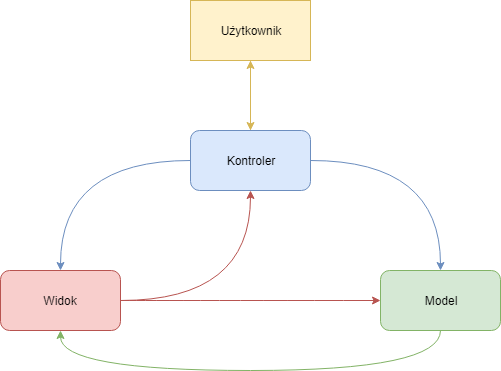
\includegraphics[scale=0.8]{mvc.png}
	\caption{Schemat klasycznego wzorca MVC}
	\label{fig:schemat_mvc}
\end{figure}
Strona internetowa powstała na bazie bardzo popularnego wśród programistów wzorca projektowego MVC. Założenia wzorca Model-Widok-Kontroler są bardzo proste, ich składowymi są:
\begin{itemize}
\item Model- reprezentuje logikę biznesową. Tutaj znajdują się wszelkie obiekty, które służą do wykonywania zaimplementowanej funkcjonalności danej aplikacji,
\item Widok- jest warstwą prezentacji. Odpowiada za prezentację logiki biznesowej (Modelu) użytkownikowi w przystępny sposób,
\item Kontroler- obsługuje żądania użytkownika. Odebrane zadania oddelegowuje do odpowiednich modeli.
\end{itemize}

\subsection{Single Page Application}
Single Page Application (SPA) to aplikacja lub strona internetowa, która w całości wczytuje się za jednym razem. Cały potrzebny do działania strony kod (HTML, CSS, JavaScript) przesyłany jest na początku lub dodawany dynamicznie w kawałkach, zwykle w odpowiedzi na interakcje generowane przez użytkownika.
Sposób działania takiej aplikacji jest zbliżony do odczuć towarzyszących korzystaniu z aplikacji desktopowej lub mobilnej.

\subsection{Chmura obliczeniowa}
\begin{figure}[H]
	\centering
	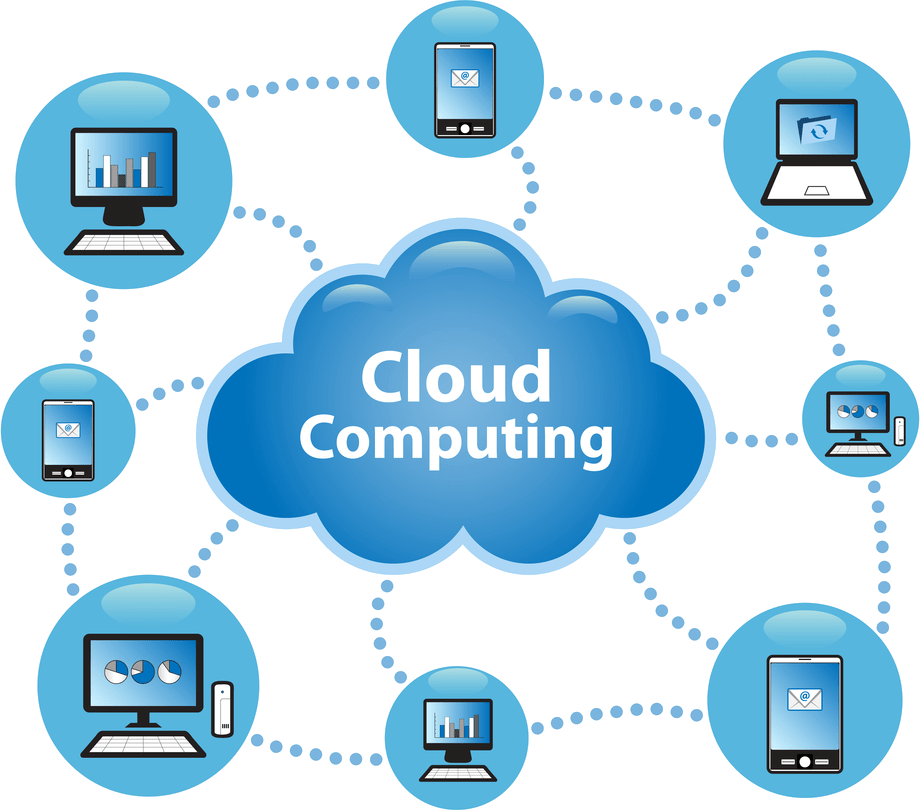
\includegraphics[scale=0.8]{cloud_computing.png}
	\caption{Obliczenia chmurowe}
	\label{fig:schemat_mvc}
\end{figure}
Chmura obliczeniowa jest określeniem oznaczającym model przetwarzania danych oparty na użytkowaniu usług dostarczonych przez usługodawcę. Użytkownik nie musi opłacać licencji, a płaci jedynie za użytkowanie danej usługi. W przypadku takich usług najpopularniejszym sposobem naliczania kosztów jest opłata od czasu użytkowania usługi.
DO najpopularniejszych udostepnianych usług należą:
\begin{itemize}
\item bazy danych,
\item maszyny wirtualne,
\item serwery,
\item hosting dla aplikacji webowych.
\end{itemize}
Przedstawicielami usługodawców udostępniających szeroki zakres usług, które zostały wykorzystane podczas tworzenia tej pracy magisterskiej jest Azure od Microsoft oraz AWS stworzony przez Amazon. Usługi obu podmiotów, które mogą być przydatne podczas tworzenia rozwiązania zostały szerzej opisane w podpunkcie \ref{azure} i \ref{aws}.
\subsection{1-Wire} \label{1wire}
One Wire to systemowa magistrala komunikacji elektronicznej pomiędzy urządzeniami, zapewniająca przesyłanie danych oraz zasilanie urządzenia przez pojedynczy kabel. Proces ten jest możliwy dzięki stopniowemu ładowaniu kondensatora znajdującego się w odbiorniku, a następnie wykorzystanie zgromadzonej energii do zasilenia urządzenia. Do magistrali może zostać podłączonych wiele urządzeń. Każdemu z nich przydzielany jest indywidualny adres 64-bitowy. Komunikację z urządzeniami inicjuje master, w tym przypadku Raspberry Pi.
Przedstawiony protokół jest bardzo podobny do I2C, ale ze względu na wykorzystanie jedynie jednej linii danych, charakteryzuje się niższą prędkością przesyłania. Układ zazwyczaj zasilany jest napięciem o wartości 5V i służy do komunikacji pomiędzy niewielkimi urządzeniami, takimi jak np. termometr cyfrowy i mikrokontroler.

\section{Raspberry Pi} \label{raspi}
Raspberry Pi jest platformą komputerową stworzoną przez Raspberry Pi Foundation, na którą składa się pojedynczy obwód drukowany. Pierwsza wersja tego urządzenia została zaprezentowana w 2012 roku. Na potrzeby tej pracy wykorzystano nowszą wersję urządzanie w wersji 3 B, którą została wyposażona w 4 rdzeniowy procesor i 1 GB pamięci RAM. Raspberry pozwala na podłączenie wielu urządzeń peryferyjnych za pomocą 4 portów USB lub 40 pinów GPIO. Dodatkowe złącze pozwala na podłączenie dedykowanej kamery. Dzięki znacznej ilości portów GPIO istnieje możliwość komunikacji cyfrowej z sensorami. Budowa urządzenia nie pozwala na podłączenie czujników analogowych.
\begin{figure}[H]
	\centering
	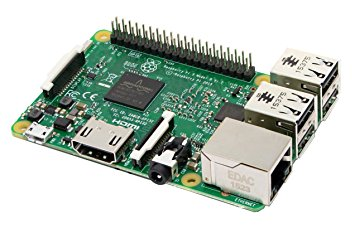
\includegraphics[scale=0.7]{raspberrypi.jpg}
	\caption{Raspberry Pi 3 B}
	\label{fig:raspberrypi}
\end{figure}

\subsection{Czujnik DHT 11}
\begin{figure}[H]
	\centering
	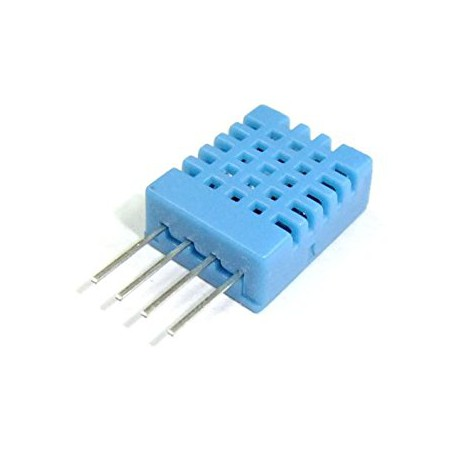
\includegraphics[scale=0.2]{dht11.jpg}
	\caption{Czujnik DHT11}
	\label{fig:dht11}
\end{figure}
Czujnik temperatury i wilgotności powietrza DHT11 jest bardzo popularnym czujnikiem z interfejsem cyfrowym. Do komunikacji wykorzystuje on protokół 1-wire opisany w rozdziale \ref{1wire}.
\begin{table}[H]
	\centering
	\caption{Parametry czujnika}
	\begin{tabular}{|c|c|}
  		\hline 
  		\bfseries Parametr & \bfseries Wartość \\
  		\hline
  		Napięcie zasilania & 3,3V do 5,5V\\
  		\hline
  		Średni pobór prądu & 0,2 mA\\
  		\hline 
  		Zakres pomiaru temperatury & od - 20\si{\degree}C do +50\si{\degree}C\\
  		\hline 
  		Zakres pomiaru wilgotności & od 5\% do 95\% wilgotności względnej\\
  		\hline 
  	\end{tabular}
\end{table}

\subsection{Raspberry Pi Camera HD}
Raspberry Pi Camera HD jest dedykowaną kamerą przeznaczoną tylko i wyłącznie do urządzenia Raspberry Pi w wersji 3, 2 oraz B+. Szybszy transfer danych niż przez port USB zapewnia dedykowane złącze minikomputera (w formie taśmy na zdjęciu \ref{fig:picamera}). Kamera posiada matrycę o rozdzielczości 8 Mpx, wspiera tryb HD 1090p, 720p oraz 640 x 480. Moduł umożliwia wykonywanie zdjęć w rozdzielczości nawet 3280 x 2464 px. Wymagane sterowniki są preinstalowane na kompatybilnych urządzeniach.
\begin{figure}[H]
	\centering
	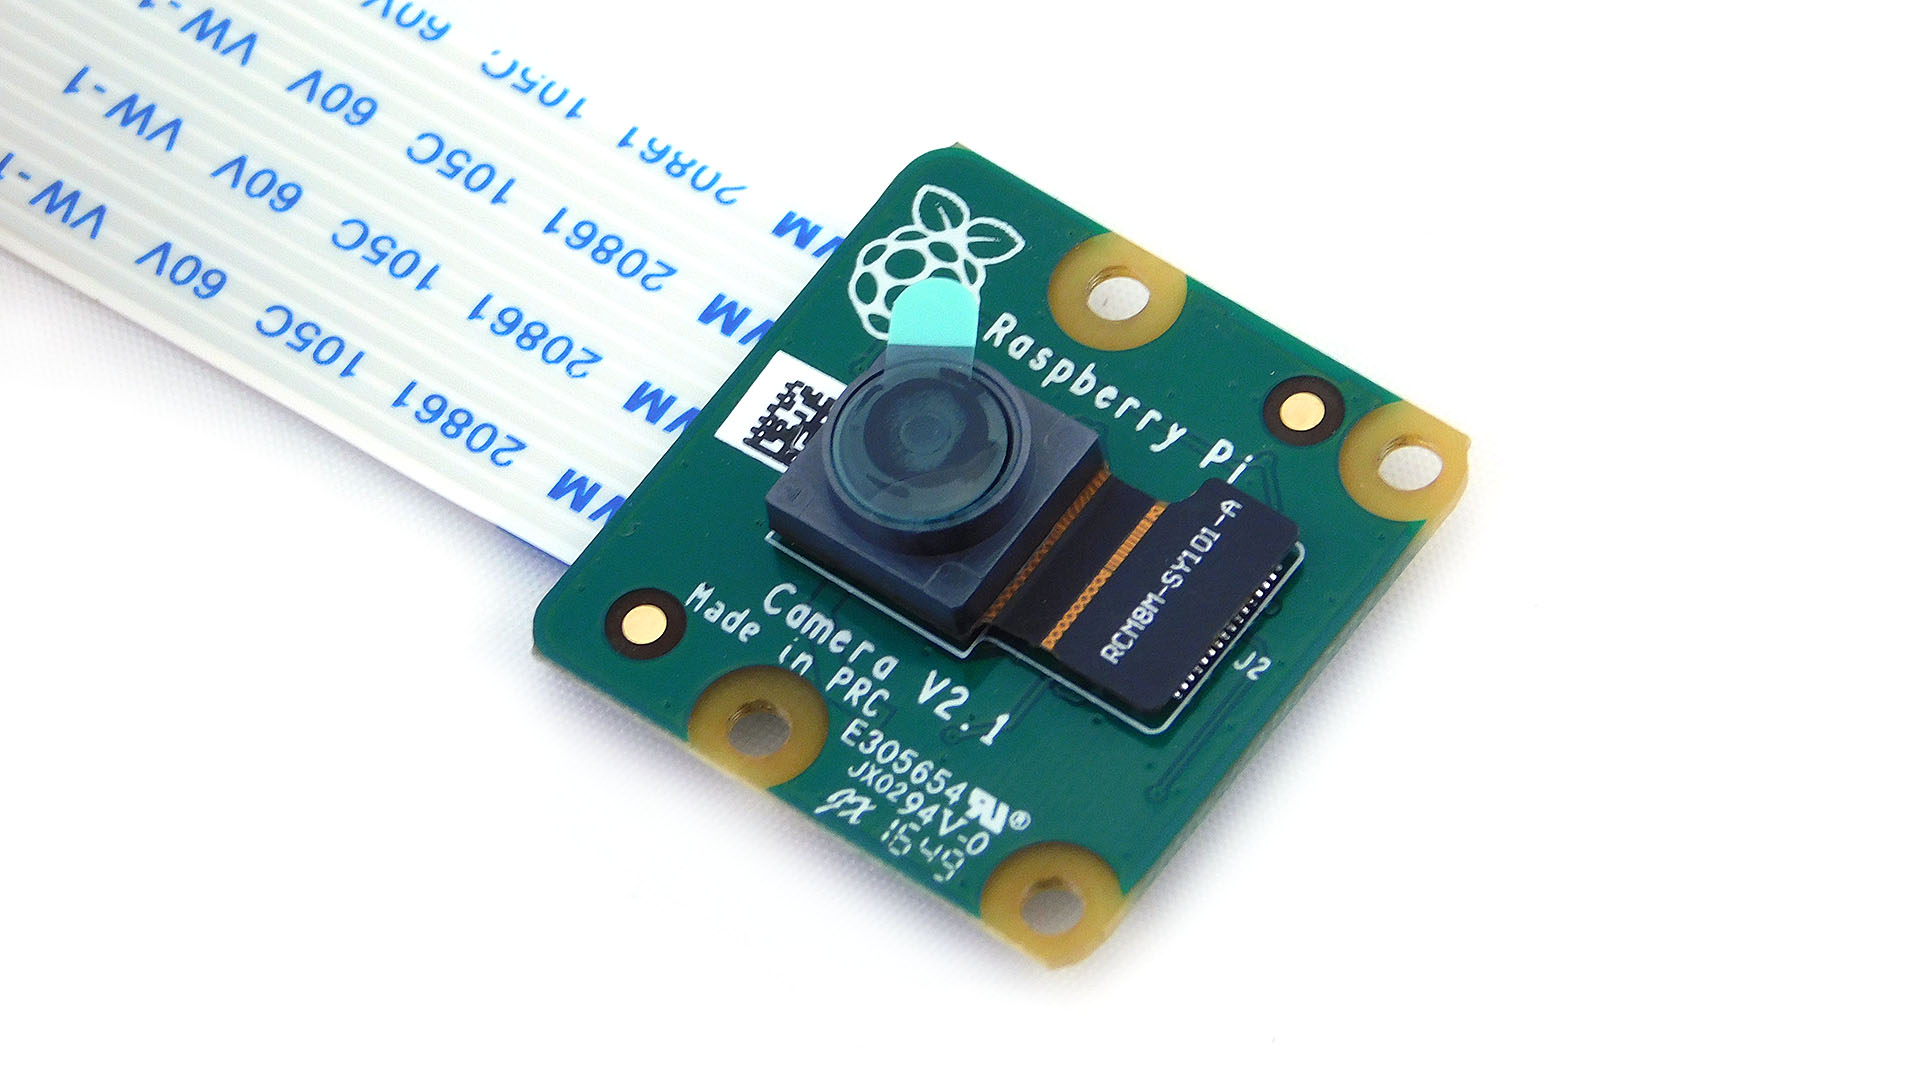
\includegraphics[scale=0.05]{picamera.jpg}
	\caption{Raspberry Pi Camera Hd}
	\label{fig:picamera}
\end{figure}

\section{Open Cv}
OpenCv (Open Source Computer Vision Library) jest open sourcową biblioteką napisaną w języku C. Udostępniono liczne interfejsy biblioteki pozwalające na pracę z nią miedzy innymi w języku C++ i Python. Biblioteka wspiera systemy operacyjne Linux oraz Windows. Biblioteka została ukierunkowana na przetwarzanie obrazu w czasie rzeczywistym. W licznie udostępnionych funkcjach można znaleźć moduły pozwalające na detekcję i rozpoznawanie twarzy na obrazie, które zostały szerzej opisane w kolejnym punkcie.

\subsection{Detekcja twarzy}
Głównym wykrywaczem twarzy wykorzystywanym przez OpenCv jest kaskadowy klasyfikator Haar'a ale poza nim istnieją również inne metody. Jedną z nich jest wykorzystanie głębokiej sieci neuronowej.

\subsubsection{Klasyfikator kaskad Haar'a} \label{haar}
Detekcja obiektów klasyfikatorem kaskad Haar'a została oparta o metodę Paul'a Viola i Michael'a Jones'a– w skrócie Viola-Jones.

\subsubsection{Algorytm Viola-Jones}
Jest to jeden z pierwszych algorytmów pozwalających na osiągnięcie zadowalających wyników w detekcji obiektów na obrazie. Został on zaproponowany w 2001 roku i został przemyślany z głównym przeznaczeniem dla detekcji twarzy. Na kluczowe koncepcje tej metody składają się:
\begin{itemize}
\item wyszukiwanie cech Haar'a,
\item integralność obrazu,
\item metoda uczenia AdaBoost (podstawowy algorytm do boostingu, metoda dzięki której z dużej liczby słabych klasyfikatorów można otrzymać jeden lepszy )
\end{itemize}

\subsubsection{Cechy Haar'a}
Cechy wykorzystywane w metodzie Viola-Jones opierają się na falkach Haara. Falki Haara są to sekwencje przeskalowanych kwadrato-podobnych funkcji, które razem tworzą falę(falo-podobną oscylację), podstawę z której można zbudować kwadrat. W dwóch wymiarach, fala kwadratu jest parą przylegających do siebie prostokątów, gdzie jeden jest jaśniejszy, a drugi ciemniejszy.
\begin{figure}[H]
	\centering
	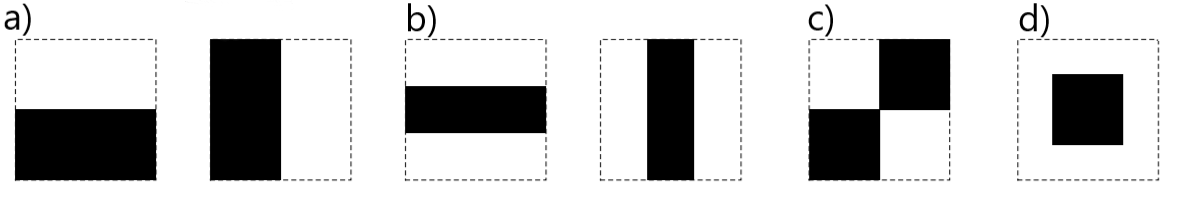
\includegraphics[scale=0.4]{szablon_cech_haara.png}
	\caption{Szablony cech Haar'a}
	\label{fig:szablon_cech_haara}
\end{figure}
Wartość każdej cechy jest obliczana jako różnica sumy poziomów szarości pikseli pokrywanych przez biały oraz czarny prostokąt oraz sumy poziomów szarości pikseli pokrywanych przez czarny prostokąt. Składniki tej różnicy posiadają wagi odwrotnie proporcjonalne do rozmiarów, dzięki czemu różnice wielkości dwóch obszarów są kompensowane.

\subsubsection{Głęboka sieć neuronowa} \label{dnn}
Pojęciem uczenia maszynowego określa się dziedzinę nauk związanych ze sztuczną inteligencją, zajmującą się badaniem algorytmów i systemów, które usprawniają swoje działanie wraz ze zdobywaniem nowej wiedzy lub też doświadczeniem. Wiedzą określamy dane uczące, które zostały wykorzystane do nauki. System może zostać usprawniony poprzez zwiększenie wiedzy systemu, które powinno pozwolić na usprawnienie procesu rozwiązywania podstawowych problemów.
\begin{figure}[H]
	\centering
	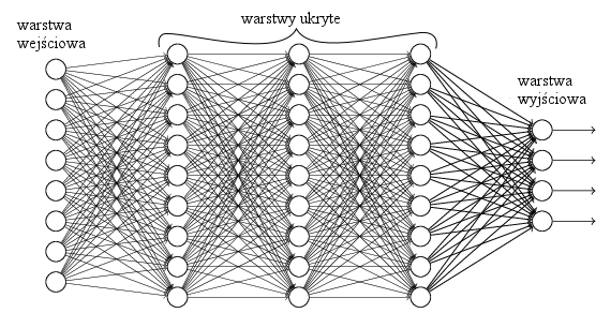
\includegraphics[scale=0.6]{schemat_dnn.png}
	\caption{Budowa głębokiej sieci neuronowej}
	\label{fig:budowa_dnn}
\end{figure}
Algorytmy głębokiego uczenia maszynowego są jednymi z najbardziej zaawansowanych. Zbudowane są one w sposób przypominający biologiczne sieci neuronowe. Głęboka sieć neuronowa składa się z neuronów rozmieszczonych na warstwach. Wiele warstw jest powodem dla którego taki rodzaj algorytmu określa się mianem głębokiego. Przykładowa budowa głębokiej sieci neuronowej została przedstawiona na rysunku \ref{fig:budowa_dnn}.

Każdy z takich “sztucznych neuronów” jest tak naprawdę informacją, która jest przesyłana dalej do następnych neuronów i ich warstw. Poszczególne warstwy “uczą” się przetwarzać kolejne cechy obiektów/obrazów/dźwięków itp., dzięki czemu są w stanie odtwarzać całe obiekty w bardzo rzeczywisty sposób.

\subsection{Rozpoznawanie twarzy \textcolor{red}{TODO}}
\subsubsection{Eigenfaces} \label{eigen}
The PCA method finds the directions with the greatest variance in the data, called principal components.
\subsubsection{Fisherfaces} \label{fisher}
\subsubsection{Local Binary Patterns Histograms} \label{lbph}

\section{Azure} \label{azure}
\subsection{App Services}
\subsection{Bazy danych SQL}
\subsection{Maszyny wirtualne}
\subsection{Azure Cognitive Services}
Cognitive Services jest częścią platformy Azure stworzonej przez Microsoft. Usługa jest standardowo płatna, ale w przypadku użytku na potrzeby studenckie przyznawany jest darmowy dostęp na ograniczony czas. Cognitive Services zajmuje się rozwiązywaniem problemów biznesowych dzięki sztucznej inteligencji. Do dostępnych modułów między innymi należą:
\begin{itemize}
\item obraz- algorytmy przetwarzania obrazów umożliwiające inteligentne identyfikowanie, podpisywanie i moderowanie grafik,
\item mowa- konwertowanie wypowiedzi audio na tekst, weryfikacja głosowa,
\item język- przetwarzanie języka naturalnego.
\end{itemize}
Na cele tego projektu wykorzystano moduł dotyczący przetwarzania obrazu, a dokładniej wykrywanie i rozpoznawanie twarzy w nim dostępne. Producent zadbał o prostą możliwość integracji z większością popularnych języków programistycznych poprzez udostępnienie paczek deweloperskich. W przypadku braku SDK dla wybranego języka istnieje możliwość skorzystania z udostępnionego REST Api. Na stronie producenta można znaleźć obszerną dokumentację oraz tutoriale.

\section{AWS} \label{aws}
\subsection{Elastic Beanstalk}
\subsection{EC2}
\subsection{RDS}
\subsection{Rekognition}

